\documentclass[journal]{IEEEtran}
\usepackage[a5paper, margin=10mm, onecolumn]{geometry}
\usepackage{lmodern}
\usepackage{tfrupee}
\setlength{\headheight}{1cm}
\setlength{\headsep}{0mm}

\usepackage{gvv-book}
\usepackage{gvv}
\usepackage{cite}
\usepackage{amsmath,amssymb,amsfonts,amsthm}
\usepackage{algorithmic}
\usepackage{graphicx}
\usepackage{textcomp}
\usepackage{xcolor}
\usepackage{txfonts}
\usepackage{listings}
\usepackage{enumitem}
\usepackage{mathtools}
\usepackage{gensymb}
\usepackage{comment}
\usepackage[breaklinks=true]{hyperref}
\usepackage{tkz-euclide}
\usepackage{listings}
\def\inputGnumericTable{}
\usepackage[latin1]{inputenc}
\usepackage{color}
\usepackage{array}
\usepackage{longtable}
\usepackage{calc}
\usepackage{multirow}
\usepackage{hhline}
\usepackage{ifthen}
\usepackage{lscape}
\usepackage{xparse}

\bibliographystyle{IEEEtran}

\title{10.7.91}
\author{EE25BTECH11043 - Nishid Khandagre}

\begin{document}
\maketitle

\renewcommand{\thefigure}{\theenumi}
\renewcommand{\thetable}{\theenumi}

\numberwithin{equation}{enumi}
\numberwithin{figure}{enumi}

\textbf{Question}:\
The point of intersection of the tangents at the ends of the latus rectum of the parabola $y^2 = 4x$ is

\textbf{Solution: }
The general form of a conic section is\\
\begin{align}
\vec{x}^{\top}\vec{V}\vec{x} + 2\vec{u}^{\top}\vec{x} + f = 0
\end{align}

    \begin{align}
    \vec{V} &= \myvec{0 & 0 \\ 0 & 1} , \vec{u}= \myvec{-2 \\ 0} ,f= 0
    \end{align}
    
Latus rectum endpoints are $\myvec{\text{a}\\\pm 2\text{a}}$\\
For $y^2 = 4x$, $a=1$.So the endpoints of the latus rectum are: $\vec{q_1} = \myvec{1 \\ 2}$,$\vec{q_2} = \myvec{1 \\ -2}$



The tangent at a point $\vec{q}$ on the conic is given by the formula:
\begin{align}
\myvec{\vec{V}\vec{q} + \vec{u}}^{\top}\vec{x} + \vec{u}^{\top}\vec{q} + f = 0 
\end{align}

    For $\vec{q_1} = \myvec{1 \\ 2}$:
    \begin{align}
    \vec{V}\vec{q_1} &= \myvec{0 & 0 \\ 0 & 1}\myvec{1 \\ 2} = \myvec{0\\ 2} \\
    \vec{V}\vec{q_1} + \vec{u} &= \myvec{0 \\ 2} + \myvec{-2 \\ 0} = \myvec{-2 \\ 2} \\
    \vec{u}^{\top}\vec{q_1} &= \myvec{-2 & 0}\myvec{1 \\ 2} = -2 \\
    f &= 0
    \end{align}
    The tangent at $\vec{q_1}$ is: 
    \begin{align}
    \myvec{-2 \\ 2}\vec{x} - 2 = 0
    \end{align}
    y = x+1. \label{eq:tangent1}

    For $\vec{q_2} = \myvec{1 \\ -2}$:
    \begin{align}
    \vec{V}\vec{q_2} &= \myvec{0 & 0 \\ 0 & 1}\myvec{1 \\ -2} = \myvec{0 \\ -2} \\
    \vec{V}\vec{q_2} + \vec{u} &= \myvec{0 \\ -2} + \myvec{-2 \\ 0} = \myvec{-2 \\ -2} \\
    \vec{u}^{\top}\vec{q_2} &= \myvec{-2 & 0}\myvec{1 \\ -2} = -2 \\
    f &= 0
    \end{align}
    The tangent at $\vec{q_2}$ is:
    \begin{align}
    \myvec{-2 \\ -2}\vec{x} - 2 = 0
     x + y + 1 = 0 \quad \Rightarrow \quad y = -x-1\label{eq:tangent2}
    \end{align}
      
      
    Intersection of the two tangents:\\
    We solve the system of linear equations from \ref{eq:tangent1} and \ref{eq:tangent2}:
    \begin{align}
    y &= x+1 \\
    y &= -x-1
    \end{align}
    Equating the right-hand sides:
    $x+1 = -x-1$
    $2x = -2$
    $x = -1$
    Substitute $x=-1$ into the first equation:
    $y = (-1) + 1 = 0$

    Therefore, the point of intersection is $\myvec{-1 \\ 0}$.

The point of intersection of the tangents at the ends of the latus rectum of the parabola $y^2 = 4x$ is $\boxed{(-1, 0)}$.

\begin{figure}[H]
\centering
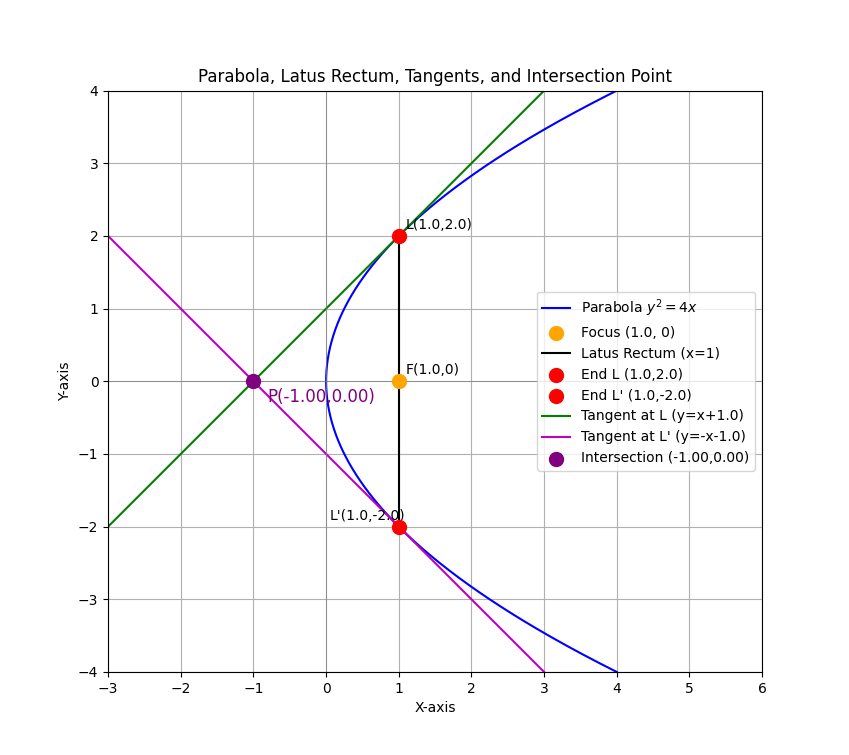
\includegraphics[width=0.7\columnwidth]{figs/mat181.png}
\caption{}
\label{fig:1}
\end{figure}

\end{document}
